%*******************************************************************************
%****************************** Second Chapter *********************************
%*******************************************************************************

\chapter{FlinkCQL- Queries over Data Stream}

\ifpdf
    \graphicspath{{Chapter4/Figs/Raster/}{Chapter4/Figs/PDF/}{Chapter4/Figs/}}
\else
    \graphicspath{{Chapter4/Figs/Vector/}{Chapter4/Figs/}}
\fi


\subsection*{Query}

A query is a request telling system what to do in order to retrieve or alter desired information stored or processed by system. For instances, asking ``How many products are sold today? ''. Queries over data stream and in a traditional DBMS have a lot in common; however, due to characteristic of continuousness in data stream, we may classify a query as one-time query or continuous query \citep{Terry:1992} \citep{Babcock:2002}. 
\begin{itemize}
	\item \textbf{One-time queries} are evaluated once over data set at a given time instant, and terminated after returning its result. This is also called \textit{passive query} \citep{SmartVotex:2011} since system require queries and passively waits for users to issue these queries before executing. 
	\item \textbf{Continuous queries}, in contrast, get evaluated continually as new data arrives to the observed stream. System continuously delivery new results  over time according to the snapshot or state of data stream seen so far. Thus the output of queries is not a single result, but rather new streams of results for further operators if desired. Obviously, continuous queries really fit to user's requirements to observed data streams till its end. 
\end{itemize}



\subsection*{Query Language}
Queries are expressed in terms of some query language. Queries provide for users and programmers a very general way to specify data selections, projections, combination, computation and so on over data set/stream. In the meanwhile, users can send the queries using either imperative or declarative language.

\subsubsection*{Imperative vs. Declarative language}
\begin{itemize}
	\item \textbf{Imperative language} requires users to define explicitly step by step \textbf{how} code should be executed to get \textbf{what} they want. They need to break the program into sequences of commands in particular order for the system to perform. Actually, many existing programming languages are imperative supporting \textit{assignemnt}, \textit{for-loop}, \textit{if-else} statements and so on to construct the complete program. For example, assuming that \textit{StockTick} is a  list of stock transactions,  to filter through \textit{StockTick} to get all stock transactions from `NYSE' only: 
\begin{lstlisting}
	function getTransFromNYSE {
		var fromNYSE = []
		for (var i = 0; i < StockTick.length; i++) {
			if (StockTick[i].Exchange == "NYSE")
				fromNYSE.add(StockTick[i])
		}
	}
\end{lstlisting}
	\item \textbf{Declarative language}, like SQL or LINQ, users just specify \textbf{what} they want - which sort of data, which transformation they want it to be afterwards, but \textbf{not how} to achieve the result. The corresponding declarative program for previous examples is written in SQL language as below:
	\begin{verbatim}
		SELECT * from StockTick where Exchange = "NYSE"
	\end{verbatim}
\end{itemize}

There are several advantages of declarative over imperative language \citep{Martin:2014}:

\begin{itemize}
	\item Declarative language is typically more concise , more friendly and easier to work with. For instance, comparing 2 previous programs, the former has 7 lines of code while the latter goes with 1 line. According to \citep{Ronnie:2015}, Java program is typically 50 times less compact than SQL query for the same purpose. Generally, that because they have different level of abstraction. Declarative language already hides complicated implementation details. It makes the program much more simpler but possible for system to introduce underneath improvement without any impact on queries.
	\item Declarative languages, for example SQL, HTML,  are usually followed a set of standard syntaxs which make it more limited in functionality, give the system more room for automatic optimization. 
	\item In terms of parallel execution environment, declarative language like SQL has a better chance to be executed faster. Imperative code instructs its sequence of operators to be performed in a certain order so that it is really hard to parallelize programs across distributed system. In the other hand, declarative queries are more atomic to be implemented in parallel if appropriate.
\end{itemize}

\subsection*{FlinkCQL - a SQL-like dialect}
Recently, there are 2 common forms of declarative language applying to data query: SQL and LINQ. However, we decide to extend SQL syntax for our continuous query language due to several advantages:
\begin{itemize}
	\item Traditional database model and data stream model are distinguished but till share many common features and operators. Since,SQL was a well-designed for handle data in batch mode, extending it to handle data-in-motion in data stream model is a possible incremental approach to quickly define language with less effort.
	\item SQL is so common and recognized by most of developers. Therefore, extended SQL languare would not challenge them to learn and master it.
	\item SQL is a standard adopted by most of relational database systems. As a result, their syntax is well-designed and refactored. Moreover, parsers, visualizers and composers for SQL are readily available to extend.
\end{itemize}

http://www.sqlstream.com/blog/2015/03/why-we-need-sql-for-real-time-streaming-analytics/

	
%\subsubsection*{LINQ}
%https://www.linqpad.net/WhyLINQBeatsSQL.aspx
%http://pankajtiwarii.blogspot.hu/2012/09/advantages-and-disadvantages-of-linq_3.html

%Despite its power, LINQ doesn't deprecate SQL. It takes more than 95 percents of the querying brunt, but you still sometimes need SQL for:

%Hand-tweaked queries (especially with optimization or locking hints)

%Queries that involve selecting into temporary tables, then querying those tables

%Predicated updates and bulk inserts

%\subsubsection*{Visual languages} \citep{Henrique:2014}


There are several properties of data stream which we take into account when extending SQL to FlinkCQL:

\begin{itemize}
	\item \textbf{Language closure}: it ensures that the output of any one query can be input to another
	\item \textbf{Windowing} FlinkCQL allow to define window specification and  implement related operators
	\item \textbf{Non-blocking operators} Naturally, blocking operation is not applicable to data stream
\end{itemize}

We are hereby going to present FlinkCQL syntax on \ref{language} and its semantic  on \ref{semantic}





In the streaming literature, query language model a stream as a representation for an infinite append-only relation. The append-only stream model effects the following limitations\citep{Ghanem:2008}
\begin{itemize}
\item It limits the applicability of the language since the append-only models cannot represent streams from the various domain( e.g., the update streams or streams that represent concatenation of the states of a fixed size relation).
\item The append-only stream model limits the types of queries that the language can express since only non-blocking queries can produce append-only streams as output
\item The semantics of query composition in the append-only stream model is complex and the meaning of the composed queries is difficult to understand.
\end{itemize}

Query \citep{Babcock:2002} 

Query : Smart Votex , page 2

Window Specification over Data Streams.pdf

[Stream] Evaluate CQL

Designing\_Data\_Intensive\_Applications.pdf



%\section{Fundamental Features}

%\begin{itemize}
%\item Stream-oriented Query Languages and Operators
%	\begin{itemize}
%		\item Language closure
%		\item Windowing
%		\item Correlation
%		\item Pattern Matching
%	\end{itemize}
	
%\item Fundamental of Stream Processing : page 110
%	\begin{itemize}
%		\item Compositional elements
%		\item Declarative operators
%		\item Expression language
%		\item Type System
%		\item Windowing
%		\item Standard operators and adapters
%		\item Modularity
%		\item Configuration
%		\item Extensiblity
%	\end{itemize}
%\end{itemize}


\section{Continuous Query Language} \label{language}

\subsection{Data Type}

FlinkCQL supports numbers of data types including numeric types (\textit{Byte}, \textit{Short}, \textit{Int}, \textit{Long}, \textit{Float}, \textit{Double}), \textit{Boolean}  type, string types (\textit{Char}, \textit{String}), deta type (\textit{Datetime}) with detailed descriptions in (Table~\ref{table:Data Type})


\begin{table}[h]
\caption{Data Type}
\centering
\label{table:Data Type}
\setlength\extrarowheight{5pt}
\begin{tabular}{||>{\centering\bfseries}m{1in} |>{\centering}m{3in}  |>{\centering\arraybackslash}m{2in}||}
\hline
%\rowcolor[HTML]{ECF4FF} 
%{\color[HTML]{ECF4FF} \textbf{Scala Type}} & {\color[HTML]{ECF4FF} \textbf{Flink Type}} & {\color[HTML]{ECF4FF} \textbf{Viewable as}} \\ \hline
\textbf{FlinkCQL Type} & \textbf{Description}  & \textbf{Convertable to} \\ \hline\hline
                    String  & A sequence of Chars                               &  \\ \hline
                    Boolean	& Either the literal true or the literal false			               &   \\ \hline
                   Char		& 16 bit unsigned Unicode character. Range from U+0000 to U+FFFF			 &  Byte, Short, Integer, Long, Double\\ \hline
					Byte		 & 8 bit signed value. Range from -128 to 127          	                   & Short, Integer, Long,Float, Double \\ \hline
					Short	& 16 bit signed value. Range -32768 to 32767			               & Integer, Long, Float, Double\\ \hline								
					Int		& 32 bit signed value. Range -2147483648 to 2147483647			 & Long, Float, Double\\ \hline
					Long		& 64 bit signed value. -9223372036854775808 to 9223372036854775807	 		                     & Float, Double \\ \hline								
					Float	& 32 bit IEEE 754 single-precision float			                    & Double \\ \hline
					Double	& 64 bit IEEE 754 double-precision float			                  &   \\ \hline							
	Datetime				&     'YYYY-MM-DD HH:MM:SS' format. The supported range is '1000-01-01 00:00:00' to '9999-12-31 23:59:59'               &        	\\ \hline           							           							           							           							           
\end{tabular}
\end{table}



\subsection{Data Definition Language (DDL)}
We utilize Extended Backus–Naur Form (EBNF) to make a formal descriptions of FlinkCQL. To understand the syntax, there are some EBNF notations to know
\begin{itemize}
	\item $\textbf{[...]}$ : Expression inside squared brackets is \textit{optional}
	\item $\textbf{\{...\}}$ : Expression, which is wrapped by curly braces, is omitted or repeated. 
	\item $\textbf{|}$ : alternation (or)
\end{itemize} 
Moreover, be aware that \textit{ident} stands for \textit{Identifier} which is recognized as name of schema, stream, data attribute and so on.
\newpage
\subsubsection{Create Schema}

%\setlength{\grammarparsep}{20pt plus 1pt minus 1pt} % increase separation between rules
\setlength{\grammarindent}{12em} % increase separation between LHS/RHS 

\begin{grammar}

<schema statement> ::= CREATE SCHEMA <schema ident> \\
(<named schema ident>|<anonymous schema>) \\
  { }[EXTENDS <parent schema ident>]

<anonymous schema> ::= `(' <typedAttribute> \{`,' <typedAttribute>\}`)'

<typedAttribute> ::= <attribute ident> <data type>

\end{grammar}
	
Similar to CREATE TABLE statement in SQL, we are able to identify a schema of stream tuples. Each schema consist of name followed by list of data attributes (the combination of attribute identifier and its data type). For example, we create schema for \textit{StockTick} stream:
\begin{verbatim}
CREATE SCHEMA StockTickSchema (symbol String, sourceTimestamp Long, 
price Double, quantity Int, exchange String)
\end{verbatim}

We extends the grammar so that a schema can be referenced or extended to another schema. For examples, in below examples, \textit{StockTickSchema2} is referencing to previous \textit{StockTickSchema} so that they own a similar set of attributes. Meanwhile, \textit{StockTickSchema3} extends from it to have one more attribute (\textit{"id"})
\begin{verbatim}
CREATE SCHEMA StockTickSchema2 StockTickSchema
CREATE SCHEMA StockTickSchema3 (id Int) EXTENDS StockTickSchema
\end{verbatim}

\subsubsection{Create Stream}
	
					
\begin{grammar}
<Stream statement> ::= CREATE STREAM <schema ident> \\		(<named schema ident>|<anonymous schema> ) \\
{ }[<source>]

<source> ::= (AS <derived source>) | ( SOURCE <raw source>)

<derived source> ::=  <stream ident>| <subSelect>

<raw source> ::= 
				HOST `('<host>, <port>`)'
					\alt FILE `('<file path>, <delimiter>`)'
\end{grammar}

A stream cannot be queried unless it is registered with a schema, simply because system require users to specify name of attributes for expression in most of cases. For this reason, we allow to entitle a stream to its schema using CREATE STREAM statement. Except for the reserved keywords, the statement consists of 3 parts. Stream name declaration is followed by schema definition and source of stream. Its schema can be recalled from a previously-defined named schema such as \textit{StockTickSchema}. 
\begin{verbatim}
CREATE STREAM StockTick StockTickSchema;
\end{verbatim}

One also has abilities to define new schema with a set of attribute name and type. In this case, the stream and its schema share the same name.
\begin{verbatim}
CREATE STREAM StockTick (symbol String, price Double, quantity Int)
\end{verbatim}

The last part is optional source of stream. Recall that we have two kind of stream representations: base stream and derived stream. \textit{<raw source>} clause indicates that this is a base stream obtained through a network connection (\textit{<host>, <post>}) or from a text file. For instance, \textit{StockTick} stream originates from host \textit{98.138.253.109} via port \textit{2000}

\begin{verbatim}
	CREATE STREAM StockTick StockTickSchema 
	SOURCE HOST ("98.138.253.109", 2000)
\end{verbatim}

Derived stream may come from another existing stream or output of a query and its operators. \textit{<derived source>} clause indicates these two possibilities. For example, we register a new stream \textit{StockPrice} which is derived from \textit{StockTick} but pay attention to stock symbol and its price only
\begin{lstlisting}
	CREATE STREAM StockPrice (symbol String, price Double) AS
	SELECT symbol, price 
	FROM StockTick
\end{lstlisting}


\subsection{Data Manipulation Language (DML)}

\subsubsection{Insert}

\begin{grammar}
<insert statement> ::= INSERT INTO <stream ident> [AS] 
							(<stream ident> | <subSelect>)
\end{grammar}
% <merge>

In CREATE STREAM statement, stream identifier and its schema definition are required but its source is optional. It means that registered stream could attached its source later when it is available. In this case, we take the advantage of INSERT statement to complete stream registration procedure. However, we support INSERT statement for derived stream only. It naturally makes sense because a base stream is concrete and should be permanently registered from beginning. We then can insert it into other stream if possible.
Keep in mind that INSERT statement is a complementary to CREATE STREAM statement in case \textit{<source>} is missing. It will not work for a stream identifier which already refer to a real stream source.

\begin{verbatim}
	CREATE STREAM StockTick StockTickSchema;
	INSERT INTO StockTick AS stockStream;
\end{verbatim}


\subsubsection{Merge}
\begin{grammar}
<merge statement> ::= MERGE <stream ident> `,' <stream ident> {`,'<stream ident>}
\end{grammar}

One of data stream properties is that data are emitted by a variety of external sources. It is cumbersome to write a similar query for each of substream. To eliminate this duplication, Flink allows to merge various registered stream with same Schema into one. For example, we integrate all StockTick from several Exchange into one:
\begin{verbatim}
	MERGE stockTickFromNYSE, stockTickFromAMEX, stockTickFromNASDAQ
\end{verbatim}


\subsubsection{Split}
\begin{grammar}
<split statement> ::= ON <stream ident> \\
						<insert clause> \{, <insert clause>\}
						
<insert clause> ::= INSERT INTO <stream ident> \\SELECT <target entry list> WHERE <predicate>
\end{grammar}

Sometimes, user would like to divide an original stream into several sub-streams according to given criteria. And hence, it is more convenient to observe changes on different sub-streams or sends further queries. Consider the following examples, we classify the original \textit{StockTick} stream and divide into 3 sub-streams based on quantity of transaction.

\begin{verbatim}
on StockTick
insert into LargeTicks select symbol, price where quantity >= 100000
insert into MediumTicks select symbol, price where quantity between 20000 and 100000
insert into SmallTicks select symbol, price where quantity > 0
\end{verbatim}

\subsubsection{Select}
\begin{grammar}
<select statement> ::= SELECT <target entry> \{, <target entry>\}\\
	FROM <stream references> \\
	WHERE <predicate> \\
	GROUP BY <attribute ident> \{,<attribute ident>\} \\
	INTO <stream ident>
	
<stream references> ::= <stream refererence> [<join clause>]

<stream reference> ::= (<stream ident>| <subSelect>) [`['Window specification`]']

<join clause> ::= CROSS JOIN <stream reference>
				\alt [INNER] JOIN <stream  reference> (ON <predicate> | USING <attribute ident>)

<window specification> ::= 
								SIZE <spec> \\
								{ }[EVERY <spec>]\\
								{ }[PARTITIONED BY <attribute ident> \{,<attribute ident>\}]

<spec> ::= <int> ON <attribute ident>
			\alt <int> <time unit>
			\alt <int>
\end{grammar}

The specification of a SELECT query in FlinkCQL resembles the formulation of one-time queries in standard SQL with common SELECT, FROM, WHERE and GROUP BY clause. However, we did enhance the FROM clause with a \textit{<window specification>} to cope with window operators. The semantic of GROUP BY  also differ from one in native SQL as well. All changes will be mentioned in details in the following:

\subsubsection*{FROM clause}
First, windowing constructs play an crucial role in stream processing and it really makes FlinkCQL distinctive. Our \textit{<window specification>} fully supports all kind of window semantics. It is made up of 3 parts: \textit{SIZE} denotes the window size, \textit{EVERY} indicates the slide size, and \textit{PARTITION BY} is to classify tuples of window into disjoint group. Recall the example in Figure~\ref{fig:winSpec} which query continuously on   windows grouped by Exchange value, over last 3 hours once every 1 hour
\begin{lstlisting}
	[
		SIZE 3 hours 
		EVERY 1 hours 
	 	PARTITIONED BY Exchange
	 ]
\end{lstlisting}

Furthermore, we assign different formulations of \textit{<spec>} for different measurement unit. Let us consider different windows:
\begin{itemize}
	\item System-timestamp-based windows: \textit{SIZE 1 min}: means that window captures all tuples last minute of system clock.
	\item Application-timestamp-based windows: \textit{SIZE 60 on sourceTimestamp}: means window size is 60 seconds based on \textit{sourceTimestamp} attribute
	\item Count-based windows: \textit{SIZE 100}: means that only last 100 tuples can be buffered in window.
\end{itemize}
Be aware that, if \textit{EVERY} clause is missing, window specification refer to a tumbling window by default.


Second, window specification has to follow a stream identifier or a sub query which producing a data stream. Consider a query which continuously computes the average value of transaction quantities in \textit{StockTick} stream using tumbling window spanning last 100 transaction:

\begin{verbatim}
	SELECT avg(quantity) FROM StockTick [SIZE 100]
\end{verbatim}

If window specification is unavailable, the query is taken place on the scope of stream which can support non-blocking operators only. For examples, the following query is invalid:
\begin{lstlisting}
	SELECT avg(quantity) FROM StockTick
\end{lstlisting}

Third, currently \textit{JOIN} and \textit{CROSS JOIN} operators are supported only on time-based windows. Temporal operators take the current windows of both streams and apply the join/cross logic on these window pairs.

The Join transformation produces a new tuple data stream with two fields. Each tuple holds a joined element of the first input data stream in the first tuple field and a matching element of the second input data stream in the second field for the current window.

The Cross transformation combines two data streams into one stream. It builds all pairwise combinations of the elements of both input data streams in the current window, i.e., it builds a temporal Cartesian product.


%\textbf{TODO}: examples in \citep{Kramer:2009} page 14
\subsubsection*{GROUP BY clause}
\textit{GROUP BY} clause in FlinkCQL have a slight different meaning agains one in SQL. This clause in native SQL is used to collect data across data set and group the results by one or more columns. System then can compute some aggregation functions in each group. However, applying \textit{GROUP BY} operator on a data stream results in several sub-streams distinguished by their ``group keys''. Since the output are streams, we are not able to apply any blocking operators on them.\textit{HAVING} clause is also not applicable in this case. However,  we may obtain a stream of partitioned windows (Figure~\ref{fig:partitionedWin}) when discretizing those sub-streams using window operators. We present here the query to compute continuously average of transaction quantities in partitioned windows at  (Figure~\ref{fig:partitionedWin})
\begin{lstlisting}
	SELECT ave(quantity)
	FROM StockTick [SIZE 2]
	GROUP BY symbol, exchange
\end{lstlisting}


\subsubsection{Operators}
\begin{enumerate}

\item Scala-based Operators
	\begin{itemize}
        \item Arithmetic
        \item Logical
        \item Comparison / Relational
        \item Bitwise
	\end{itemize}
	
 \item List and Range Operators
 	\begin{itemize}
        \item In / Not in
        \item Between
        \item Null
 	\end{itemize}
 \item String Operators
 	\begin{itemize}
        \item Like
        \item Regex
 	\end{itemize}
 \item Function 
 	\begin{itemize}
        \item Aggregate Func
        \item Coversion Func
       	\item Data and Time Func
        \item String func
 	\end{itemize}

\end{enumerate}
Semantic and Implementation of Continuous Sliding window queries over data streams

[thesis] CQL over data stream [BNF] alias



\section{Continuous Query Semantics and Operators} \label{semantic}
Semantics of Data Streams and Operators

%\href{http://en.wikipedia.org/wiki/Relational\_algebra}{http://en.wikipedia.org/wiki/Relational\_algebra}

\subsection*{Streams and Relations}
As we mentioned, it is nearly impossible to perform non-blocking operators on data streams due to its infinity or velocity. However, those operators usually bring up many useful and concise insights about the recent state of the stream such as joining, aggregation and so on. Stream processing engine offers windowing techniques to restrict the scope of the operators to a finite set of elements from underlying stream. The set of tuples within a window is really closed to concept of relations in traditional database system in terms of 
\begin{itemize}
	\item the size of data set is finite so that system can perform all relation-to-relation operators on it.
	\item Each element of data set belongs to a predefined Schema.
	\item The order of elements is not a matter, since most of non-blocking operators treat every element equally. 
\end{itemize} 

For that reason, the concept of relation in data stream was first proposed in CQL \citep{Arasu:2006} for further analysis. 

\begin{defi}
	A relation R is a partial function mapping from each time instant $t \in \mathbb{T}$ to a finite but unbound set of tuples belonging to the schema of R.
\end{defi}

In our model, we make a clear different between application and system timestamp. $R(t_{app} = \tau)$ denotes an unordered set of tuples at any application time instant $\tau$ in a condition that $R(t_{app} = -1) = \emptyset$ since function $f$ is not defined. $R(t_{sys} = \tau)$ also implies the tuple at the system time instant if existing because there is at most one tuples at that given time instant. 

Querying operators on FlinkCQL falls into 4 classes (Figure~\ref{fig:relation}):
\begin{itemize}
	\item \textbf{Stream-to-Relation} operators: are based on windowing technique. It takes a stream as an input then produces a relation. System continuously buffers and reflects the interested part of the stream as a relation for further process. Relation of a window can be thought of as the set of all tuples within the window.
	\item  \textbf{Relation-to-Relation} operators: produce a output relation from one or more input relations. The operators are directly inherited from the standard SQL operators as a whole.
	\item \textbf{Relation-to-Stream} operator is responsible for producing a output stream from a input relation. Flink provides a flatten function to unwrap a windows and convert a windowed stream to normal data stream. Thanks to this function, FlinkCQL perform a single Relation-To-Stream right after finishing \textit{projection} operator (specified on SELECT clause), and produce a new output stream.
	\item \textbf{Stream-to-Stream} operators: Three of previous operator classes is fully support in CQL. However, it does not support direct operators between stream. To do so, system transforms a stream into relation, perform a chain of relational operators then convert back to stream format. In contrast, Flink allows to transform directly from input streams to output streams on all non-blocking operators and preserves the order of elements in stream.
\end{itemize}
\begin{figure}[htbp!] 
\centering    
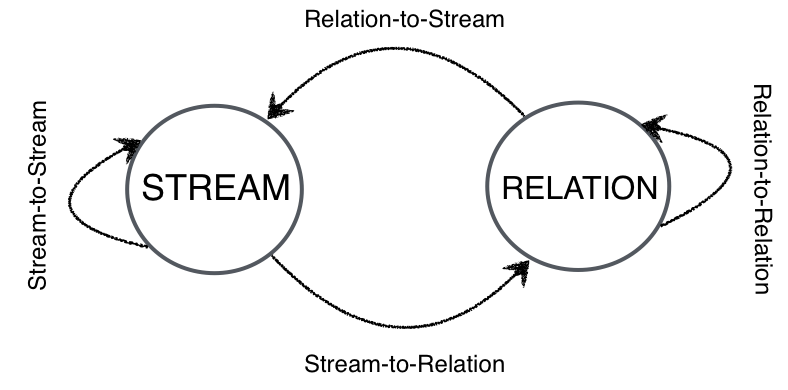
\includegraphics[width=0.7\textwidth]{relation}
\caption{FlinkCQL operators}
\label{fig:relation}
\end{figure}


%\subsection*{Denotation Language}
%\subsection*{Lamda Calculus}
%\subsection{Abstract Syntax}
%\subsection{Domain}
%\subsection{Denotation Semantics}


\subsection*{Stream-to-Stream}
\begin{enumerate}
	\item Projection
	
	$\mathcal{M}_{S2S}\sembrack{Select(A_1,A_2,..,A_k)} \\
		{}\qquad= \lambda_S.\{<(v.A_1,v.A_2,...,v.A_k),\tau_{app},\tau_{sys}>: \forall s<v,\tau_{app},\tau_{sys}>\in S \\
		{}\qquad\land (A_1,A_2,..,A_k) \subset Schema \}$ 
		
	\item Selection
	
	$\mathcal{M}_{S2S}\sembrack{Where(p)} \\
		{}\qquad= \lambda_S.\{s: \forall s \in S  \land p(s.v) = true \}$ 
		
	\item Merge/Union
	$\mathcal{M}_{S2S}\sembrack{Merge} \\
		{}\qquad= \lambda_{S_1}\lambda_{S_1}...\lambda_{S_k}.\{s: s \in S_1 \lor s \in S_1 \lor ... \lor s \in S_k \}$ 
	
	\item Split
	$\mathcal{M}_{S2S}\sembrack{Split} \\
		{}\qquad= \lambda_{S}.\lambda_{f}.\{s: s \in S \land f(s.v) = true \}$ 
	\item Grouping
	
	$\mathcal{M}_{S2S}\sembrack{GroupBy(A_1,A_2,..,A_k)} \\
		{}\qquad= \lambda_S.\lambda_{a_1}.\lambda_{a_2}...\lambda_{a_k}.\{s: s \in S  \land  s.v.A_i= a_i \,for\, \forall i \in [1,k]\\
		{}\qquad\land (A_1,A_2,..,A_k) \subset Schema \}$ 
\end{enumerate}

\subsection*{Stream-to-Relation}
\begin{enumerate}
	\item Application-time based
	$\mathcal{M}_{S2R}\sembrack{Size\, T\, on\, A} \\
		{}\qquad= \lambda_S.\lambda_{t_{app}}\{v:  s<v,t_{app}',t_{sys}> \in S  \land t'_{app} = v.A \\
		{}\qquad max(T-t_{app},0) < t'_{app} \leq t_{app} \}$ 
		
	\item System-time based
	
	$\mathcal{M}_{S2R}\sembrack{Size\, T\, milliseconds} \\
		{}\qquad= \lambda_S.\lambda_{t_{sys}}.\{v:  s<v,t_{app},t'_{sys}> \in S  \land 
		max(T-t_{sys},0) < t'_{sys} \leq t_{sys} \}$ 
		
	\item Count-based
	
	$\mathcal{M}_{S2R}\sembrack{Size\, N} \\
		{}\qquad= \lambda_S.\lambda_{t_{sys}}\{v:  s<v,t_{app},t'_{sys}> \in S  \land (t'_{sys} \leq t_{sys}) \\
		{}\qquad \land (N \geqslant |\{<e'',t''_{app},t''_{sys}> \in S: t'_{sys} \leq t''_{sys} \leq t_{sys}\}|) \}$
\end{enumerate}

\subsection*{Relation-to-Relation}
\begin{enumerate}
		
	\item Production
	
	$\mathcal{M}_{R2R}\sembrack{CrossJoin} \\
		{}\qquad= \lambda_{t_{sys}}.\lambda_{t_{sys}}.\{(e_1,e_2) : e_1 \in E_1 \land e_2 \in E_2 \}$
		
	\item Join
	
	$\mathcal{M}_{R2R}\sembrack{InnerJoin(a,b)} \\
		{}\qquad= \lambda_{E_1}.\lambda_{E_2}.\{(e_1,e_2) : e_1 \in E_1 \land e_2 \in E_2 \land e_1.a = e_2.b \land a \in Schema(e_1) \\
		{}\qquad= \land b \in Schema(e_2) \}$
		
	\item Grouping
	
		$\mathcal{M}_{R2R}\sembrack{GroupBy(A_1,A_2,..,A_k) Selection(AggFunc)} \\
		{}\qquad= \lambda_E.\lambda_{a_1}.\lambda_{a_2}...\lambda_{a_k}.\{AggFunc(E)  \land  \forall e \in E, \,\forall i \in [1,k] e.A_i= a_i \, \\
		{}\qquad\land (A_1,A_2,..,A_k) \subset Schema(e) \}$ 
	
	\item Projection
	
		$\mathcal{M}_{R2R}\sembrack{Select(A_1,A_2,..,A_k)} \\
		{}\qquad= \lambda_E.\{(e.A_1,e.A_2,...,e.A_k):e \in E \\
		{}\qquad\land (A_1,A_2,..,A_k) \subset Schema(e) \}$
	
\end{enumerate}

\subsection*{Relation-to-Stream}
%$\mathcal{M}_{R2S}\sembrack{IStream} \\
%		{}\qquad= \lambda_R.\lambda_{t_{sys}}.\{v:  s<v,t_{app},t'_{sys}> \in S  \land 
%		max(T-t_{sys},0) < t'_{sys} \leq t_{sys} \}$ 



